\documentclass[UTF8,a4paper,8pt]{ctexbook} 

 \usepackage{graphicx}%学习插入图
 \usepackage{verbatim}%学习注释多行
 \usepackage{booktabs}%表格
 \usepackage{geometry}%图片
 \usepackage{amsmath} 
 \usepackage{amssymb}
 \usepackage{listings}%代码
 \usepackage{xcolor}  %颜色
 \usepackage{enumitem}%列表格式
 \usepackage{hyperref}
 \CTEXsetup[format+={\flushleft}]{section}


\geometry{left=1.6cm,right=1.8cm,top=2cm,bottom=1.7cm} %设置文章宽度
\graphicspath{{figure/}}

\pagestyle{plain} 		  %设置页面布局
\author{\kaishu 郑华}
\title{\heiti OpenGL4.3  学习笔记}
%代码效果定义
\definecolor{mygreen}{rgb}{0,0.6,0}
\definecolor{mygray}{rgb}{0.5,0.5,0.5}
\definecolor{mymauve}{rgb}{0.58,0,0.82}
\lstset{ %
	backgroundcolor=\color{white},   % choose the background color
	basicstyle=\footnotesize\ttfamily,        % size of fonts used for the code
	%stringstyle=\color{codepurple},
	%basicstyle=\footnotesize,
	%breakatwhitespace=false,         
	%breaklines=true,                 
	%captionpos=b,                    
	%keepspaces=true,                 
	%numbers=left,                    
	%numbersep=5pt,                  
	%showspaces=false,                
	%showstringspaces=false,
	%showtabs=false,        
	columns=fullflexible,
	breaklines=true,                 % automatic line breaking only at whitespace
	captionpos=b,                    % sets the caption-position to bottom
	tabsize=4,
	commentstyle=\color{mygreen},    % comment style
	escapeinside={\%*}{*)},          % if you want to add LaTeX within your code
	keywordstyle=\color{blue},       % keyword style
	stringstyle=\color{mymauve}\ttfamily,     % string literal style
	frame=single,					%tb top and bottom; L left double line
	xleftmargin=.06\textwidth, 
	%xrightmargin=.1\textwidth,
	rulesepcolor=\color{red!20!green!20!blue!20},
	% identifierstyle=\color{red},
	language=c++,
}

\begin{document}          %正文排版开始
 	\maketitle
 
	\newpage
	\tableofcontents
	
\newpage
\chapter{安装配置}
    \section{各种库文件}网盘环境
    \textbf{有时一个warnning可能就会导致全局皆输。}
    
    比如这次环境的调试程序,一个warnning4005  就是隐式转类型警告,结果就是跑不出来。最后发现是OpenGL为了兼容各系统,估计是把每个类型的字节固定了,而且还是32位,而我的是64位,导致了程序的不可运行
    
    \section{常见错误}
	    \subsection{0x70000000C}见图\ref{Glut Error},图\ref{Glut_fix}.
	    
		    解决:1- 使用glut.h , 2- 给链接输入添加\verb|glut32.lib Opengl32.lib Glu32.lib glew32.lib comctl32.lib|
		    \begin{figure}[h]
		    	\begin{center}
					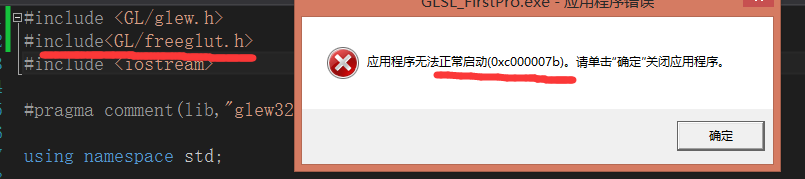
\includegraphics[scale = 0.5]{glutDoesNotMatchError.png}%就在前面括号中写图片名
		    		\caption{Error}
		    		\label{Glut Error}
		    	\end{center}
		    \end{figure}
		    \begin{figure}[h]
		    	\centering
		    	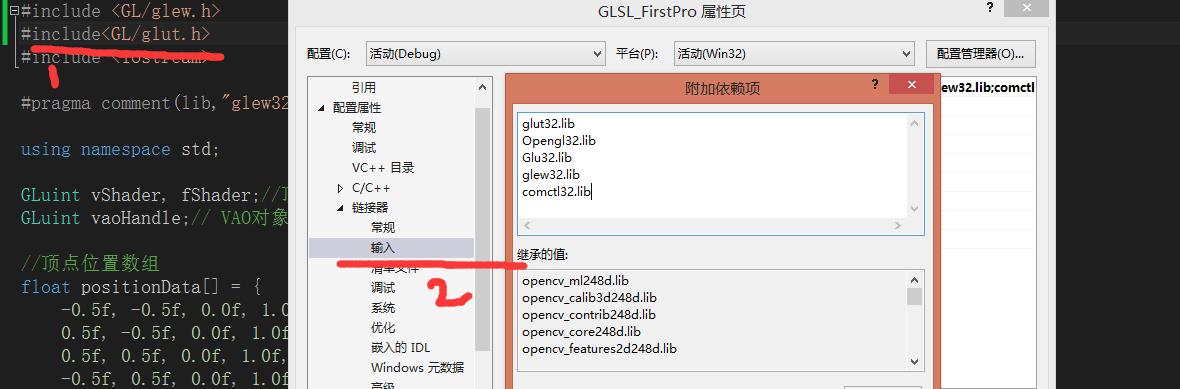
\includegraphics[scale = 0.4]{glutMatch.png}
		    	\caption{解决方法}
		    	\label{Glut_fix}
		    \end{figure}
    \section{参考文献} 
    \url{http://johnhany.net/2015/03/environment-for-opengl-4-with-vs2012/}    

\newpage
\chapter{入门绘图}
	\section{第一个三角形}
		这篇教程中我们依然使用那个单位化的盒子模型。可见的点必须在这个盒子内,这样他们将可以通过视窗的变换映射到窗口中可见的坐标上。当俯视Z坐标轴的负方向时这个单位化盒子看上去如下图:
			\begin{figure}[htbp]
				\begin{center}
					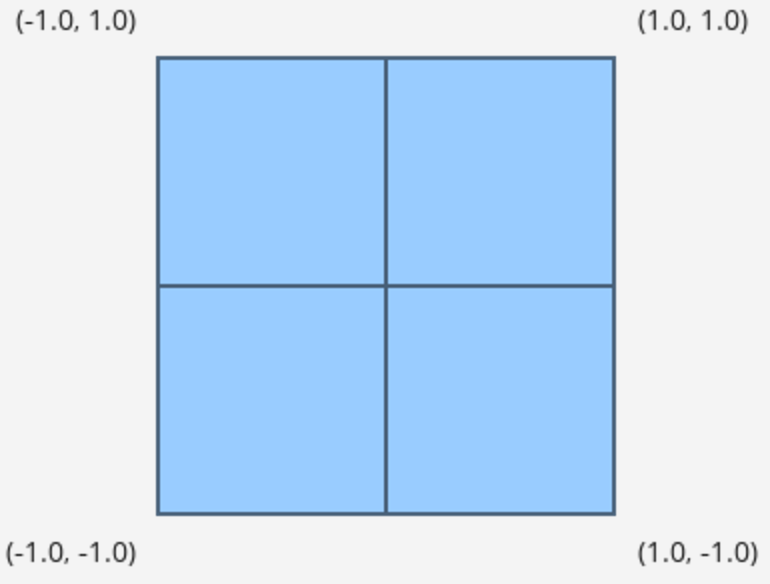
\includegraphics[scale = 0.5]{unitPic.png}
					\caption{单位示例}
				\end{center}
			\end{figure}
			
		点(-1.0, -1.0)映射到盒子的左下角,(-1.0,1.0)映射到左上角等等。如果将三角形的顶点往盒子外扩展移到盒子外,这个三角形将会被裁剪,只能看到三角形的一部分。
    
    
	   \subparagraph{核心代码}\verb|-|
	   
		  \verb|顶点数据->|  
		  \begin{lstlisting}
	Vector3f Vertices[3]; 
	Vertices[0] = Vector3f(-1.0f, -1.0f, 0.0f); 
	Vertices[1] = Vector3f(1.0f, -1.0f, 0.0f); 
	Vertices[2] = Vector3f(0.0f, 1.0f, 0.0f); 
		  \end{lstlisting} 
		  
		  \verb|绘图方式|
		  \begin{lstlisting}
	glDrawArrays(GL_TRIANGLES, 0, 3); 
		  \end{lstlisting}
		  
		  
		  \verb|示例代码|
		  \begin{lstlisting}
	#include <stdio.h>
	#include <GL/glew.h>        // GLEW扩展库
	#include <GLUT/freeglut.h>  // freeGLUT图形库
	#include "ogldev_math_3d.h" // 用于OpenGL的3d数学库
	
	GLuint VBO;
	
	/**
	* 渲染回调函数
	*/
	static void RenderScenceCB(){
		// 清空颜色缓存
		glClear(GL_COLOR_BUFFER_BIT);
		
		// 开启顶点属性
		glEnableVertexAttribArray(0);
		// 绑定GL_ARRAY_BUFFER缓冲器
		glBindBuffer(GL_ARRAY_BUFFER, VBO);
		// 告诉管线怎样解析bufer中的数据
		glVertexAttribPointer(0, 3, GL_FLOAT, GL_FALSE, 0, 0);
		
		// 开始绘制几何图形(绘制一个三角形,三个顶点)
		glDrawArrays(GL_TRIANGLES, 0, 3);
		
		//  禁用顶点数据
		glDisableVertexAttribArray(0);
		
		// 交换前后缓存
		glutSwapBuffers();
		
		glFlush();
	}
	
	/**
	* 创建顶点缓冲器
	*/
	static void CreateVertexBuffer()
	{
		// 创建含有3个顶点的顶点数组
		Vector3f Vertices[3];
		// 三角形的三个顶点位置
		Vertices[0] = Vector3f(-1.0f, -1.0f, 0.0f);
		Vertices[1] = Vector3f(1.0f, -1.0f, 0.0f);
		Vertices[2] = Vector3f(0.0f, 1.0f, 0.0f);
		
		// 创建缓冲器
		glGenBuffers(1, &VBO);
		// 绑定GL_ARRAY_BUFFER缓冲器
		glBindBuffer(GL_ARRAY_BUFFER, VBO);
		// 绑定顶点数据
		glBufferData(GL_ARRAY_BUFFER, sizeof(Vertices), Vertices, GL_STATIC_DRAW);
	}
	
	/**
	* 主函数
	*/
	int main(int argc, char ** argv) {
		
		// 初始化GLUT
		glutInit(&argc, argv);
		
		// 显示模式:双缓冲、RGBA
		glutInitDisplayMode(GLUT_DOUBLE | GLUT_RGBA);
		
		// 窗口设置
		glutInitWindowSize(480, 320);      // 窗口尺寸
		glutInitWindowPosition(100, 100);  // 窗口位置
		glutCreateWindow("Tutorial 03");   // 窗口标题
		
		// 开始渲染
		glutDisplayFunc(RenderScenceCB);
		
		// 缓存清空后的颜色值
		glClearColor(0.0f, 0.0f, 0.0f, 0.0f);
		
		// 检查GLEW是否就绪,必须要在GLUT初始化之后!
		GLenum res = glewInit();
		if (res != GLEW_OK) {
			fprintf(stderr, "Error: '%s'\n", glewGetErrorString(res));
			return 1;
		}
		
		// 创建顶点缓冲器
		CreateVertexBuffer();
		
		// 通知开始GLUT的内部循环
		glutMainLoop();
		
		return 0;
	}
		  \end{lstlisting}
	
	\section{渲染管线}
		\subparagraph{参考}\url{http://blog.csdn.net/cjneo/article/details/50538033}
		\begin{figure}[h]
			\centering
			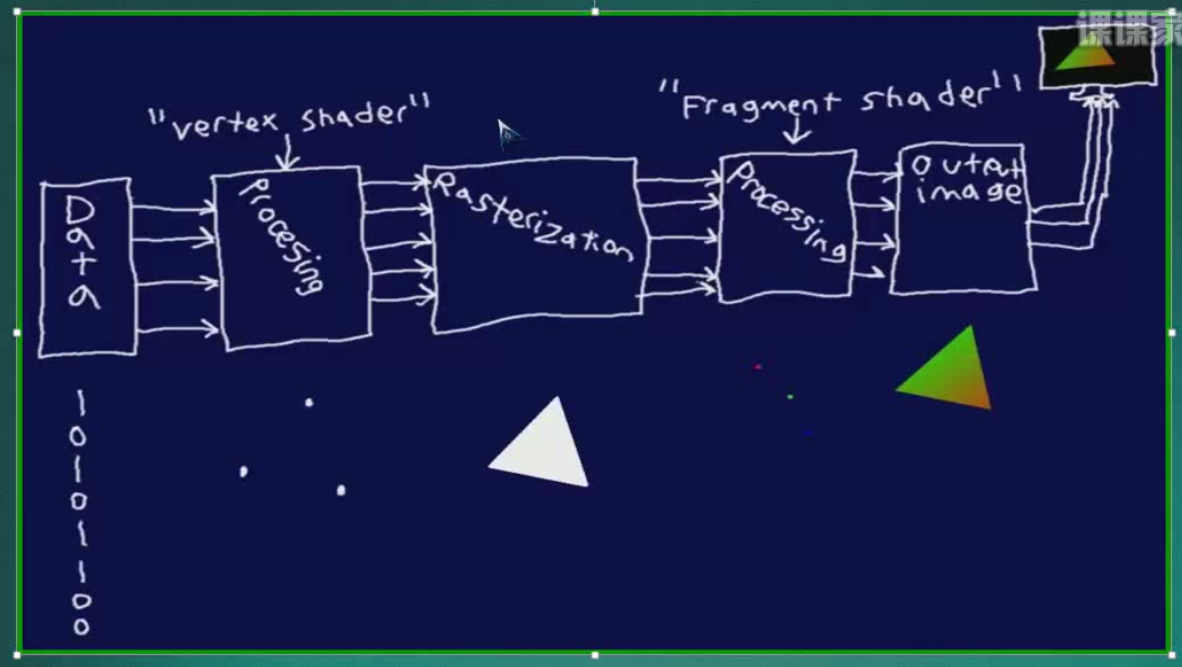
\includegraphics[scale = 0.4]{OpenGLPipeline.png}
			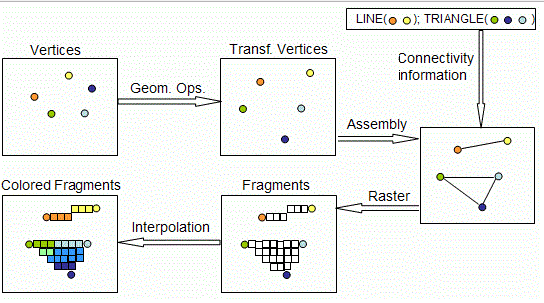
\includegraphics[scale = 0.8]{OpenGLPipeline1.png}
			\caption{OpenGL 渲染管线}
		\end{figure}
	
		\begin{enumerate}
			\item \textbf{Vertex Processor数据}:顶点数据、索引数据\verb|->|负责执行处理经过管线的每一个顶点的vertex shader顶点着色代码
			
				\verb|--|这里顶点着色器还不知道渲染的图元的topology拓扑结构是怎样的,另外不可以在顶点着色处理器阶段删除丢弃顶点,每个顶点有且只有一次经过顶点处理器,要经过变换后继续进入管线的下一步。
				
			\item \textbf{Geometry Processor顶点渲染}:链接成具体的图形拓扑结构,如点、线、面
			
			\item \textbf{Clipper}:它将所有图元裁剪到那个单位化的盒子模型内,它另外还会将图元裁剪在Z轴的远近平面范围内(也就是说太远或太近都不显示)。同时也提供用户自定义的裁剪平面进行自定义的裁剪。经过裁剪后保留下来的顶点现在会被映射到屏幕空间坐标系上,光栅器将会根据他们的拓扑结构把他们渲染到屏幕上。
			
				\verb|--|这一步更像是视图变换,选取出可以显示的部分。
				
			\item \textbf{Fragment Shader}:顶点颜色、输出带色图形[默认白色]
		\end{enumerate}
	
		上面这三个可编程阶段(vertex processor顶点处理、geometry processor几何处理、fragment processor像素处理)\textbf{都是可选的而不是必须}的。
		
		\textbf{如果不在这几个处理器上绑定自己的shaer着色器},那么就会执行一些默认的函数功能,也就是备胎着色器。
		  
	\section{着色器}
		参考文献:\url{http://blog.csdn.net/column/details/13062.html}
		
		着色器是目前做3D图形最流行的方式。着色器使得开发者能更加自由的通过编程实现自己的图形效果,使开发更加灵活和具有创新性。
			
		\textbf{Shader着色器}的使用跟C/C++程序的创建过程类似。
		\textbf{首先}你要\textit{写一个shader着色器文本}并使其在你的程序中有效可用,这个过程可以通过依次简单的引用这些源码脚本或者从外部文件中加载,注意都是以字符串数组的形式。
		\textbf{然后}一个个的\textit{编译这些shader文本}成shader对象。
		\textbf{最后}你就可以\textit{将这些shader着色器}\textbf{连接到}\textit{单个程序中并加载到GPU中}。链接这些shader可以使驱动器能够有机会精减这些shader并根据他们的关系优化他们。例如:可能一个顶点着色器发出的法向量在相应的片段着色器阶段中被忽视,这样驱动中的GLSL编译器就会移除着色器中与这个法向量相关的函数功能从而更快的执行这个顶点着色器。如果之后那个着色器又匹配了需要用到那个法向量的片段着色器,然后连接到其他程序后会产生一个不同的顶点着色器。  

		\subparagraph{核心流程}
		
			\begin{itemize}
			\item \verb|创建着色器程序对象|:我们通过\textbf{创建程序对象}\textit{来建立}\textbf{shader着色器程序}。我们将把所有的着色器连接到这个对象上。
			\begin{lstlisting}
	GLuint ShaderProgram = glCreateProgram();
			\end{lstlisting}
			
			\item \verb|创建着色器对象|:使用下面的函数创建两个shader着色器对象。其中一个使用的ShaderType为\verb|GL_VERTEX_SHADER|,另一个的类型为\verb|GL_FRAGMENT_SHADER|。
			\begin{lstlisting}
	GLuint ShaderObj = glCreateShader(ShaderType); 
			\end{lstlisting}
			
			\item \verb|定义着色器对象代码源|:函数\verb|glShaderSource|以\textbf{shader对象}为参数,使你可以灵活的定义代码来源。shader源代码(也就是我们所常说的shader脚本)可以由多个字符串数组排布组合而成,你需要提供一个指针数组来对应指向这些字符串数组,同时要提供一个整型数组来对应表示每个数组的长度。为了简单,我们这里只使用一个字符串数组来保存所有的shader源代码,并且分别用数组的一个元素来分别指向这个字符串数组和表示数组的长度。 
			第二个参数表示的是这两个数组的元素个数(我们的例子中则只有1个)。
			\begin{lstlisting}
	const GLchar* p[1]; 
	p[0] = pShaderText; 
	GLint Lengths[1]; 
	Lengths[0]= strlen(pShaderText); 
	glShaderSource(ShaderObj, 1, p, Lengths);
			\end{lstlisting}
			
			\item \verb|编译着色器对象|
			\begin{lstlisting}
	glCompileShader(ShaderObj); 
			\end{lstlisting}	
			
			\item \verb|打印编译信息|
			\begin{lstlisting}
	GLint success; 
	glGetShaderiv(ShaderObj, GL_COMPILE_STATUS, &success); 
	if (!success) 
	{ 
		GLchar InfoLog[1024]; 
		glGetShaderInfoLog(ShaderObj, sizeof(InfoLog), NULL, InfoLog); 
		fprintf(stderr, "Error compiling shader type %d: '%s'\n", ShaderType, InfoLog); 
	} 
			\end{lstlisting}
		
			\item \verb|绑定着色器对象到着色器程序对象上|
			\begin{lstlisting}
	glAttachShader(ShaderProgram, ShaderObj);
			\end{lstlisting}
			
			
			\item \verb|链接所有的编译的对象|:编译好所有的shader对象并将他们绑定到程序中后我就可以连接他们了。
			
			注意在完成程序的连接后你可以通过调用函数glDetachShader和glDeleteShader来清除每个中介shader对象。OpenGL保存着由它产生的多数对象的引用计数,如果一个shader对象被创建后又被删除的话驱动程序也会同时清除掉它,但是如果他被绑定在程序上,只调用glDeleteShader函数只是会标记它等待删除,只有等你调用glDetachShader后它的引用计数才会被置零然后被移除掉。
			\begin{lstlisting}
	glLinkProgram(ShaderProgram); 
			\end{lstlisting}
			
			\item \verb|获取链接编译信息|:如同程序的链接信息一样 LNK,我们使用glGetProgramiv而不是glGetShaderiv,glGetProgramInfoLog而不是glGetShaderInfoLog。
			\begin{lstlisting}
	glGetProgramiv(ShaderProgram, GL_LINK_STATUS, &Success); 
	if (Success == 0) 
	{ 
		glGetProgramInfoLog(ShaderProgram, sizeof(ErrorLog), NULL, ErrorLog); 
		fprintf(stderr, "Error linking shader program: '%s'\n", ErrorLog); 
	} 
			\end{lstlisting}
			
			\item \verb|使用回调函数完成渲染|:要使用连接好的shader程序你需要用下面的回调函数将它设置到管线声明中。这个程序将在所有的draw call中一直生效直到你用另一个替换掉它或者使用glUseProgram指令将其置NULL明确地禁用它。如果你创建的shader程序只包含一种类型的shader(只是为某一个阶段添加的自定义shader),那么在其他阶段的该操作将会使用它们默认的固定功能操作。
			
			到现在我们已经完成了OpenGL中和shader相关操作的准备工作的学习。在这篇教程之后的内容主要是关于顶点着色器和片段着色器(包含在pVS和pFS脚本中)。
			\begin{lstlisting}
	glUseProgram(ShaderProgram); 
			\end{lstlisting}
		\end{itemize}
		
		\subparagraph{示例}\verb|着色器使用示例|
		
			\begin{lstlisting}
	GLuint VBO;
	
	// 定义要读取的顶点着色器脚本和片断着色器脚本的文件名,作为文件读取路径(这样的话shader.vs和shader.fs文件要放到工程的根目录下,保证下面定义的是这两个文件的文件路径)
	const char* pVSFileName = "shader.vs";
	const char* pFSFileName = "shader.fs";
	
	static void RenderSceneCB()
	{
		glClear(GL_COLOR_BUFFER_BIT);
		
		glEnableVertexAttribArray(0);
		glBindBuffer(GL_ARRAY_BUFFER, VBO);
		glVertexAttribPointer(0, 3, GL_FLOAT, GL_FALSE, 0, 0);
		
		// 依然还是绘制一个三角形
		glDrawArrays(GL_TRIANGLES, 0, 3);
		
		glDisableVertexAttribArray(0);
		
		glutSwapBuffers();
	}
	
	
	static void InitializeGlutCallbacks()
	{
		glutDisplayFunc(RenderSceneCB);
	}
	
	static void CreateVertexBuffer()
	{
		Vector3f Vertices[3];
		Vertices[0] = Vector3f(-1.0f, -1.0f, 0.0f);
		Vertices[1] = Vector3f(1.0f, -1.0f, 0.0f);
		Vertices[2] = Vector3f(0.0f, 1.0f, 0.0f);
		
		glGenBuffers(1, &VBO);
		glBindBuffer(GL_ARRAY_BUFFER, VBO);
		glBufferData(GL_ARRAY_BUFFER, sizeof(Vertices), Vertices, GL_STATIC_DRAW);
	}
	
	// 使用shader文本编译shader对象,并绑定shader都想到着色器程序中
	static void AddShader(GLuint ShaderProgram, const char* pShaderText, GLenum ShaderType)
	{
		// 根据shader类型参数定义两个shader对象
		GLuint ShaderObj = glCreateShader(ShaderType);
		// 检查是否定义成功
		if (ShaderObj == 0) {
			fprintf(stderr, "Error creating shader type %d\n", ShaderType);
			exit(0);
		}
		
		// 定义shader的代码源
		const GLchar* p[1];
		p[0] = pShaderText;
		GLint Lengths[1];
		Lengths[0]= strlen(pShaderText);
		glShaderSource(ShaderObj, 1, p, Lengths);
		glCompileShader(ShaderObj);// 编译shader对象
		
		// 检查和shader相关的错误
		GLint success;
		glGetShaderiv(ShaderObj, GL_COMPILE_STATUS, &success);
		if (!success) {
			GLchar InfoLog[1024];
			glGetShaderInfoLog(ShaderObj, 1024, NULL, InfoLog);
			fprintf(stderr, "Error compiling shader type %d: '%s'\n", ShaderType, InfoLog);
			exit(1);
		}
		
		// 将编译好的shader对象绑定到program object程序对象上
		glAttachShader(ShaderProgram, ShaderObj);
	}
	
	// 编译着色器函数
	static void CompileShaders()
	{
		// 创建着色器程序
		GLuint ShaderProgram = glCreateProgram();
		// 检查是否创建成功
		if (ShaderProgram == 0) {
			fprintf(stderr, "Error creating shader program\n");
			exit(1);
		}
		
		// 存储着色器文本的字符串缓冲
		string vs, fs;
		// 分别读取着色器文件中的文本到字符串缓冲区
		if (!ReadFile(pVSFileName, vs)) {
			exit(1);
		};
		if (!ReadFile(pFSFileName, fs)) {
			exit(1);
		};
		
		// 添加顶点着色器和片段着色器
		AddShader(ShaderProgram, vs.c_str(), GL_VERTEX_SHADER);
		AddShader(ShaderProgram, fs.c_str(), GL_FRAGMENT_SHADER);
		
		// 链接shader着色器程序,并检查程序相关错误
		GLint Success = 0;
		GLchar ErrorLog[1024] = { 0 };
		glLinkProgram(ShaderProgram);
		glGetProgramiv(ShaderProgram, GL_LINK_STATUS, &Success);
		if (Success == 0) {
			glGetProgramInfoLog(ShaderProgram, sizeof(ErrorLog), NULL, ErrorLog);
			fprintf(stderr, "Error linking shader program: '%s'\n", ErrorLog);
			exit(1);
		}
		
		// 检查验证在当前的管线状态程序是否可以被执行
		glValidateProgram(ShaderProgram);
		glGetProgramiv(ShaderProgram, GL_VALIDATE_STATUS, &Success);
		if (!Success) {
			glGetProgramInfoLog(ShaderProgram, sizeof(ErrorLog), NULL, ErrorLog);
			fprintf(stderr, "Invalid shader program: '%s'\n", ErrorLog);
			exit(1);
		}
		
		// 设置到管线声明中来使用上面成功建立的shader程序
		glUseProgram(ShaderProgram);
	}
	
	// 主函数
	int main(int argc, char** argv)
	{
		glutInit(&argc, argv);
		glutInitDisplayMode(GLUT_DOUBLE|GLUT_RGB);
		glutInitWindowSize(1024, 768);
		glutInitWindowPosition(100, 100);
		glutCreateWindow("Tutorial 04");
		
		InitializeGlutCallbacks();
		
		// 必须在glut初始化后!
		GLenum res = glewInit();
		if (res != GLEW_OK) {
			fprintf(stderr, "Error: '%s'\n", glewGetErrorString(res));
			return 1;
		}
		
		printf("GL version: %s\n", glGetString(GL_VERSION));
		
		glClearColor(0.0f, 0.0f, 0.0f, 0.0f);
		
		CreateVertexBuffer();
		
		// 编译着色器
		CompileShaders();
		
		glutMainLoop();
		
		return 0;
	}
			\end{lstlisting}

		顶点着色器shader.vs脚本代码:
		\begin{lstlisting}
	#version 330  //告诉编译器我们的目标GLSL编译器版本是3.3
	
	layout (location = 0) in vec3 Position; // 绑定定点属性名和属性,方式二缓冲属性和shader属性对应映射
	
	void main()
	{
		gl_Position = vec4(0.5 * Position.x, 0.5 * Position.y, Position.z, 1.0); // 为glVertexAttributePointer提供返回值
	}		
		\end{lstlisting}
		
		片段着色器shader.fs脚本代码:
		\begin{lstlisting}
	#version 330  //告诉编译器我们的目标GLSL编译器版本是3.3
	
	out vec4 FragColor;  // 片段着色器的输出颜色变量
	
	// 着色器的唯一入口函数
	void main()
	{
		// 定义输出颜色值(R G B 透明度)
		FragColor = vec4(1.0, 0.0, 0.0, 1.0);
	}	
		\end{lstlisting}
		
		\begin{figure}[h]
			\centering
			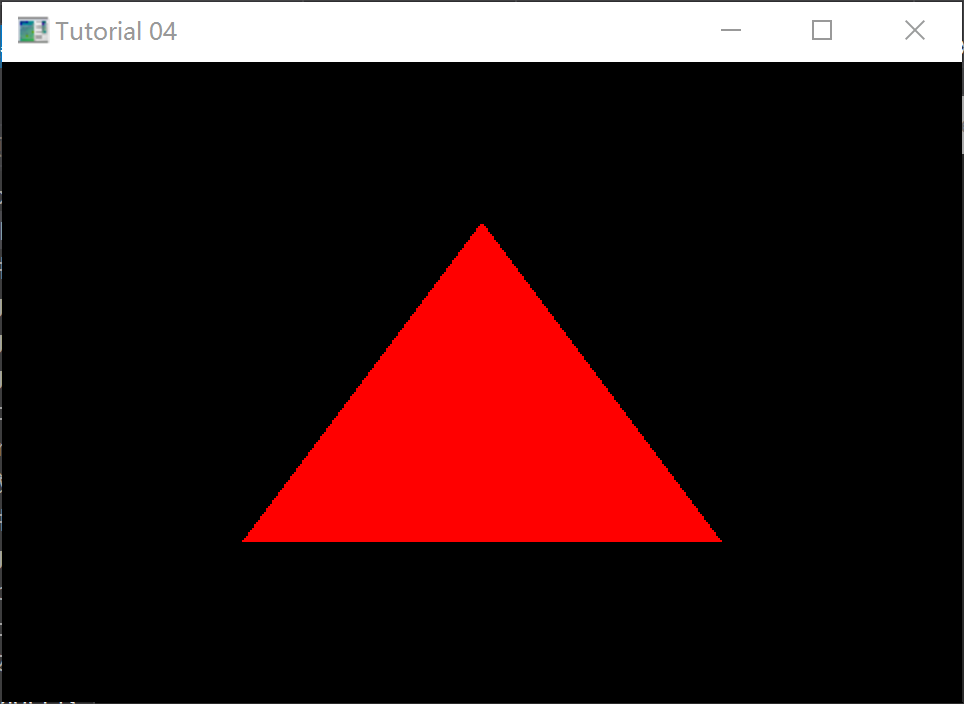
\includegraphics[scale = 0.4]{result.png}
			\caption{OpenGL 渲染管线}
		\end{figure}
		

		\subsection{顶点着色器}
			\subparagraph{主要功能}
				\begin{itemize}[itemindent = 1em]
					\item 顶点法线变换及单位化
					\item 纹理坐标变换
					\item 光照参数生成
				\end{itemize}
			\subparagraph{输入内容}
				\begin{itemize}[itemindent = 1em]
					\item 着色器源代码
					\item attribute变量
					\item uniform变量
				\end{itemize}
			\subparagraph{输出内容}
				\begin{itemize}[itemindent = 1em]
					\item varying变量
					\item 内置的特殊变量,如\verb|gl_Position、gl_FrontFacing、gl_PointSize|
				\end{itemize}
		\subsection{片段着色器}
			\subparagraph{主要功能}
				\begin{itemize}[itemindent = 1em]
					\item 在差值得到的值上进行操作
					\item 访问纹理
					\item 应用纹理
					\item 雾化
					\item 颜色融合
				\end{itemize}
			\subparagraph{输入内容}
				\begin{itemize}[itemindent = 1em]
					\item 着色器源代码
					\item 用户自定义的varying变量
					\item uniform变量
					\item 采样器(Sampler)
					\item 一些内置的特殊变量(\verb|gl_PointCoord、gl_FragCoord、gl_FrontFacing等)|	
				\end{itemize}
			\subparagraph{输出内容}:内置的特殊变量\verb|gl_FragColor|
			
		\subsection{程序组成}
			在OpenGL程序中\textbf{使用着色器}一般需要依次执行以下步骤:
			\begin{enumerate}[itemindent = 1em]
				\item 顶点着色程序的源代码和片段着色程序的源代码分别写入到一个文件里(或字符数组)里面,一般顶点着色器源码文件后缀为\textbf{.vert},片段着色器源码文件后缀为\textbf{.frag}
				\item \textbf{使用glCreateshader()}分别创建一个顶点着色器对象和一个片段着色器对象
				\item \textbf{使用glShaderSource()}分别将顶点/片段着色程序的源代码字符数组绑定到顶点/片段着色器对象上
				\item \textbf{使用glCompileShader()}分别编译顶点着色器和片段着色器对象(最好检查一下编译的成功与否)
				\item \textbf{使用glCreaterProgram()}创建一个着色程序对象
				\item \textbf{使用glAttachShader()}将顶点和片段着色器对象附件到需要着色的程序对象上
				\item \textbf{使用glLinkProgram()}分别将顶点和片段着色器和着色程序执行链接生成一个可执行程序(最好检查一下链接的成功与否)
				\item \textbf{使用glUseProgram()}将OpenGL渲染管道切换到着色器模式,并使用当前的着色器进行渲染
			\end{enumerate}	
		
			\textbf{整体流程}如下所示:
			\begin{figure}[htbp]
				\centering
				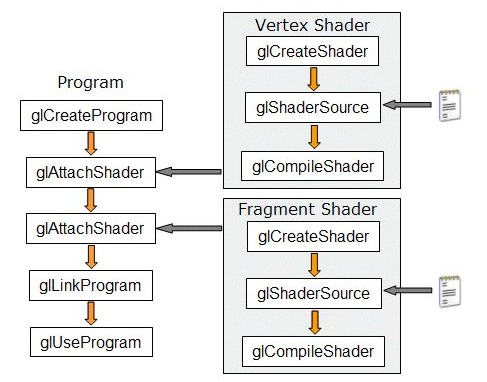
\includegraphics[width = 12cm, height = 6cm]{GLSLProcess.png}
				\caption{GLSL 流程}
				\label{GLSL}
			\end{figure}
			
			\begin{itemize}[itemindent = 1em]
				\item 准备\textbf{原始顶点数据}
				\item 准备\textbf{着色器代码}
				\item \textbf{创建着色器对象}
				\item \textbf{创建着色器程序对象}
				\item \textbf{链接着色器程序对象与着色器对象}
				\item \textbf{在程序中使用着色器}
			\end{itemize}	


\chapter{三大变换}
	从这个教程开始我们开始研究各种各样的图形变换,\textbf{图形变换就可以让一个3d物体在屏幕中变换的的时候看上去保持有深度的错觉},也就是立体的投影效果。
	
	\textbf{实现}立体效果的\textbf{方法是}使用一个\textbf{经过多次相乘的变换矩阵}得到的\textbf{最终变换矩阵}来\textbf{和顶点的位置再相乘},\textit{这样得到3d物体的一个多次变换后的最终复合变换效果}。
	
	\section{平移}
		参考文献:\url{https://blog.csdn.net/cordova/article/details/52541902}
		
		为了实现平移转换\textbf{所以矩阵是4*4的}
		
		
		这里我们先看一下平移变换,使一个物体沿着一个任意长度任意方向的向量平移,比如说让一个三角形从左边移动到右边:
			\begin{figure}[h]
				\centering
				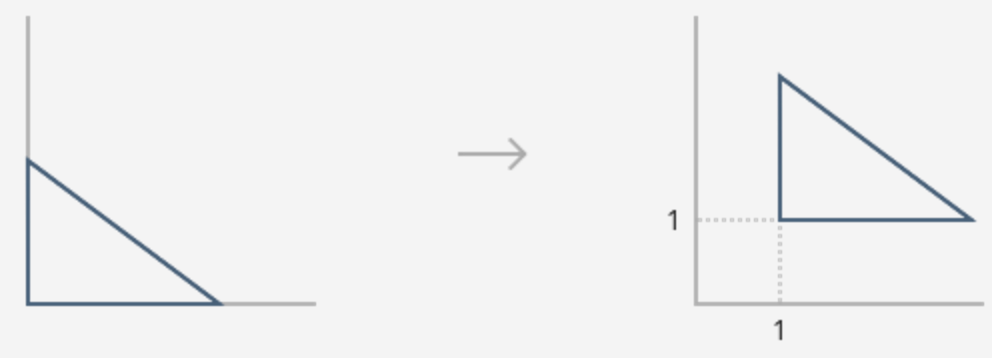
\includegraphics[scale = 0.4]{transfer.png}
				\caption{平移示例}
			\end{figure}

		在之前顶点着色器知识的基础上我们可以想到实现平移的一种办法是设置一个偏移向量(这里就是- 1了),并把这个便宜向量定义成一致变量然后传递给shader让每一个顶点按照那个偏移向量移动即可。
		
		但这样就\textit{打破}\textbf{通过乘以一个经过多个变换矩阵相乘得到的复合变换矩阵来进行复合变换}\textit{的统一性了}。
		 
		统一的说,我们是想找到这样一个矩阵,对于给定的\verb|点P(x,y,z)|和平移向量$V(v1,v2,v3)$,能够使 $M * P = P1(x+v1, y+v2, z+v3) $,简单地说就是\verb|矩阵M将P转换成了P+V|。在结果向量\verb|P1|中我们可以看到每个分量是\verb|P|和\verb|V|每个分量对应相加的和,结果向量P1的+号左侧来自P本身,对于得到P本身的向量应该这样: 
		\verb|I * P = P(x,y,z)| 。所以我们应该从得到本身开始来调整变换矩阵得到结果矩阵右侧相加结果(…+V1, …+V2, …+V3)的最终变换矩阵。首先自身变换矩阵的样子如下:
			\begin{equation}
			 \left(
			\begin{array}{ccc}
			1 & 0 & 0\\
			
			0 & 1 & 0\\
			
			0 & 0 & 1\\
			\end{array}
			\right)
			\left(
			\begin{array}{c}
				X\\ 
				Y\\
				Z 
			\end{array}	
			\right) 
			=
			\left(
				\begin{array}{c}
				X\\ 
				Y\\
				Z 
				\end{array}	
			\right)
		\end{equation}
		
		我们想修改这个自身变换矩阵使结果变成这样子:
			$$
				\left(
				\begin{array}{c}
				X+V_1\\ 
				Y+V_2\\
				Z+V_3 
				\end{array}	
				\right)
			$$
		
		如果我们坚持用$3\times3$矩阵好像不可能得到想要的结果,但如果改成$4\times4$矩阵我可以这样得到想要的结果:
			\begin{equation}
			\left(
			\begin{array}{cccc}
			1 & 0 & 0& V_1\\
			
			0 & 1 & 0& V_2\\
			
			0 & 0 & 1& V_3\\
			
			0 & 0 & 0& 1\\
			\end{array}
			\right)
			\left(
			\begin{array}{c}
			X\\ 
			Y\\
			Z\\
			1 
			\end{array}	
			\right) 
			=
			\left(
			\begin{array}{c}
			X+V_1\\ 
			Y+V_2\\
			Z+V_3\\
			1 
			\end{array}	
			\right)
			\end{equation}
		
		这样使用一个4维向量表示一个3维向量叫做\textbf{齐次坐标},这在3d图形学中很常用也很有用,第四个分量称作\verb|“w”|。事实上,我们之前教程中看到的内部shader符号变量\verb|gl_Position|就是一个4维向量,第四个分量\verb|“w”|在从3d到2d的投影变换中起着关键作用。通常对于表示点的矩阵会让\verb|w=1|,而对于表示向量的矩阵会让\verb|w=0|,\textbf{因为点可以被做变换而向量不可以},你可以改变一个向量的长度和方向,但是长度和方向一样的所有向量都是相等的,不管他们的起点在哪里,所以我们可以把所有的向量起点放到原点来看。对于向量设置\verb|w=0|然后乘以\textbf{变换矩阵}会得到\textbf{和自身一样的向量}。
		
	\section{旋转}
		参考文献:\url{https://blog.csdn.net/cordova/article/details/52558133}
		
		旋转变换将总是改变位置的其中两个坐标,第三个坐标保持不变,这意味着旋转的路径会保持在其中一个平面上:XY平面(绕Z轴旋转),YZ平面(绕X轴旋转)和XZ平面(绕Y轴旋转)。也有一些复杂的旋转变换允许图形绕着任意向量旋转,但在我们这个阶段还不需要。
		
		让我们从普遍统一的角度来定义这个问题。看下面这个图:
			\begin{figure}[h]
				\centering
				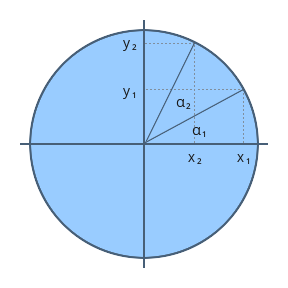
\includegraphics[scale = 0.7]{rotate.png}
				\caption{旋转示例}
			\end{figure}
		
		我们想从(x1,y1)沿着圆移动到(x2,y2),换句话说就是将点(x1,y1)旋转a2角度。假设圆的半径是1,那有下面的式子:
		\begin{equation}
			\begin{cases}
				x_1 = cos(\alpha_1)\\
				y_1 = sin(\alpha_1)\\
				x_2 = cos(\alpha_1 + \alpha_2)\\
				y_2 = sin(\alpha_1 + \alpha_2)
			\end{cases}
		\end{equation}
		
		我们用下面的三角函数变换公式来推导x2和y2的表达式:
		$$
			\begin{cases}
				cos(\alpha_1 + \alpha_2) = cos(\alpha_1)\cdot cos(\alpha_2) - sin(\alpha_1)\cdot sin(\alpha_2)\\
				sin(\alpha_1 + \alpha_2) = sin(\alpha_1)\cdot cos(\alpha_2) + cos(\alpha_1)\cdot sin(\alpha_2)
			\end{cases}
		$$
		
		上式等价于
		$$
		\begin{cases}
			x_2 = x_1\cdot cos(\alpha_2) - y_1\cdot sin(\alpha_2)\\
			y_2 = y_1\cdot cos(\alpha_2) + x_1\cdot sin(\alpha_2)
		\end{cases}
		$$
		
		
		再上面的图中我们看的是XY平面,Z轴指向纸面。X和Y放在4维矩阵里面的的话那么上面的公式可以写成下面的矩阵形式(不影响Z和W分量):
		
		\begin{equation}
		\left(
		\begin{array}{cccc}
		cos(\alpha_2) & -sin(\alpha_2) & 0& V_1\\
		
		sin(\alpha_2) & cos(\alpha_2) & 0& V_2\\
		
		0 & 0 & 1& V_3\\
		
		0 & 0 & 0& 1\\
		\end{array}
		\right)
		\left(
		\begin{array}{c}
		X\\ 
		Y\\
		Z\\
		1 
		\end{array}	
		\right) 
		=
		\left(
		\begin{array}{c}
		x_1\cdot cos(\alpha_2) - y_1\cdot sin(\alpha_2)\\ 
		y_1\cdot cos(\alpha_2) + x_1\cdot sin(\alpha_2)\\
		Z+V_3\\
		1 
		\end{array}	
		\right)
		\end{equation}
	\section{缩放}
		参考文献:\url{https://blog.csdn.net/cordova/article/details/52558804}

		缩放变换非常简单,它的目的是增大或者缩小物体的尺寸。比如你想使用同一个模型来制作很多不同的物体(大小不一的树组成的树林,用的同一个模型),或者你想按照比例让物体和现实世界尺寸一致。在上面的情形中你就需要在三个坐标轴上同等缩放顶点的位置。当然,有时也希望物体只在一个轴上或者两个轴上缩放使模型更薄、更瘦或者更高等等。
		
		进行缩放变换其实很简单。我们从最开始的原变换矩阵来看,回忆平移变换矩阵的样子,我们保持结果矩阵中V1,V2和V3保持原样的办法是让变换矩阵主对角线上的值都为’1’,这样原向量一次都和1相乘之后依然保持不变,各分量之间互不影响。所以,这里的缩放变换,只要把那些‘1’换成我们想缩放的值,原向量各分量分别乘以这些值之后就会在相应坐标轴上进行相应的缩放了,值大于1则放大,值小于1则缩小。
		
		\begin{figure}[h]
			\centering
			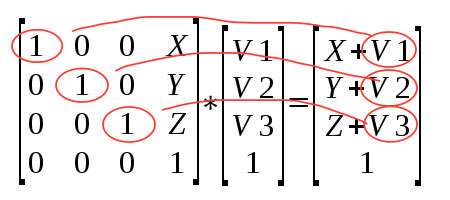
\includegraphics[scale = 0.57]{scale_1.png}
			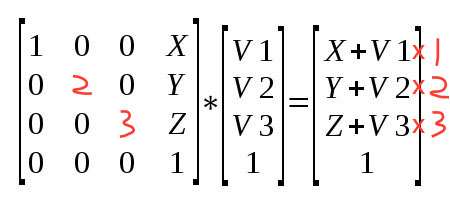
\includegraphics[scale = 0.57]{scale_2.png}
			\caption{缩放示例}
		\end{figure}

\chapter{四大变换}
参考文献:\url{http://blog.csdn.net/lyx2007825/article/details/8792475}



   
\chapter{OpenGL基础编程}
	
	\subsection{基本结构-框架}
		跟DirectX类似,都是进入消息循环然后不断监听消息。区别在于函数名可能不同,与其内部实现不同。
		有几个概念也是特别重要,其实这些就是数据准备过程和绘画过程,即Preparing to Send Data to OpenGL 和 Sending Data to OpenGL
		
		\begin{itemize}
			\item  顶点缓存对象(\textbf{Vertex Buffer Object,简称 VBO}[存在于内存中])
			\item  顶点缓存和索引缓存
			\item  缓存对象
			\item  reder()即display()
			\item 顶点数组对象 VAO (vertex array object)[显卡编程]
		\end{itemize}
		
		\subsubsection{创建顶点缓存}
			\begin{enumerate}
				\item 创建缓存对象,使用 glGenBuffers()
				\item 绑定缓存对象(指定使用哪一个缓存对象),使用 glBindBuffer()
				\item 拷贝顶点数据到缓存对象中,使用 glBufferData()
			\end{enumerate}
			
			\subparagraph{- void glGenBuffers(GLsizei n, GLuint* ids)}创建缓存对象,并返回缓存对象的标识符
				\begin{itemize}
					\item n :创建缓存对象的数量
					\item ids: 是一个 GLuint 型的变量或数组,用于储存缓存对象的单个 ID 或多个 ID
				\end{itemize}
				
			\subparagraph{- void glBindBuffer(GLenum target, GLuint id)}创建了缓存对象后,我们需要绑定缓存对象,以便使用。绑定,也就是指定当前要使用哪一个缓存对象,类似与DirectX的setStreamSource.
				\begin{itemize}
					\item target :缓存对象要存储的数据类型,只有两个值: GL\_ARRAY\_BUFFER, 和 GL\_ELEMENT\_ARRAY\_BUFFER。如果是顶点的相关属性,例如: 顶点坐标、纹理坐标、法线向量、颜色数组等,要使用 GL\_ARRAY\_BUFFER;索引数组,要使用 GL\_ELEMENT\_ARRAY\_BUFFER,以便 glDrawElements() 使用。
					
					\item id: 缓存对象的 ID
				\end{itemize}
			
			\subparagraph{- void glBufferData(GLenum target, GLsizei size, const void* data, GLenum usage)}拷贝数据到缓存对象,类似与DirectX的Lock操作.
				\begin{itemize}
					\item target: 缓存对象的类型,只有两个值: GL\_ARRAY\_BUFFER 和 GL\_ELEMENT\_ARRAY\_BUFFER
					
					\item size: 数组 data 的大小,单位是字节(bytes)
					\item data: 数组 data 的指针,如果指定为 NULL,则 VBO 只创建一个相应大小的缓存对象
					\item usage: 缓存对象如何被使用,有三中: 静态的(static)、动态的(dynamic)和流(stream).共有 9 个值:
						\begin{enumerate}
							\item GL\_STATIC\_DRAW
							\item GL\_STATIC\_READ
							\item GL\_STATIC\_COPY
							\item GL\_DYNAMIC\_DRAW
							\item GL\_DYNAMIC\_READ
							\item GL\_DYNAMIC\_COPY
							\item GL\_STREAM\_DRAW
							\item GL\_STREAM\_READ
							\item GL\_STREAM\_COPY
						\end{enumerate}
						
						\begin{itemize}
							\item Static: 指在缓存对象中的数据不能够更改(设定一次,使用很多次)
							\item Dynamic: 指数据将会频繁地更改(反复设定和使用)
							\item Stream: 指的是每一帧数据都会更改(设定一次,使用一次)
						\end{itemize}
						
						\begin{itemize}
							\item Draw: 指数据将会被送到 GPU 被用于绘制(application to GL)
							\item Read: 指数据将被读取到客户端应用程序(GL to application)
							\item Copy: 指数据将被用于绘制和读取(GL to GL)
						\end{itemize}
					\item 注意: Draw 只对 VBO 有用; Copy 和 Read 只对 PBO(像素缓存对象) 和 FBO(帧缓存对象) 有意义
				\end{itemize}
			
			\subparagraph{- void glBufferSubData(GLenum target, GLint offset, GLsizei size, void* data)}与 glBufferData() 一样,都是用于拷贝数据到缓存对象的。它能拷贝一段数据到一个已经存在的缓存,偏移量为 offset
			
			\subparagraph{- void glDeleteBuffers(GLsizei n, const GLuint* ids)}删除一个或多个缓存对象。
		
		
		\subsubsection{顶点缓存和索引缓存的使用}
			\subparagraph{1.准备顶点数据与索引数据}概念如同DirectX的绘制
				\begin{lstlisting}
	//顶点数据
	GLfloat vertexs[] = { 0.0f, 0.0f, 0.0f, 0.2f, 0.0f, 0.0f,
	-0.2f, 0.0f, 0.0f, 0.0f, 0.2f, 0.0f,
	0.0f, -0.2f, 0.0f, 0.0f, 0.0f, 0.2f,
	0.0f, 0.0f, -0.2f};
	
	//索引数据
	GLubyte indexs[] = {0,1,2,3,4,5,6};				
				\end{lstlisting}
			
			\subparagraph{2.生成缓存[数据,索引]对象,并拷贝数据}示例
				\begin{lstlisting}
	GLuint vboVertexId;
	GLuint vboIndexId;
	
	//生成数据缓存对象
	glGenBuffers(1, &vboVertexId);
	glBindBuffer(GL_ARRAY_BUFFER, vboVertexId);
	glBufferData(GL_ARRAY_BUFFER, sizeof(vertexs), vertexs, GL_STATIC_DRAW);
	
	//生成索引缓存对象
	glGenBuffers(1, &vboIndexId);
	glBindBuffer(GL_ELEMENT_ARRAY_BUFFER, vboIndexId);
	glBufferData(GL_ELEMENT_ARRAY_BUFFER, sizeof(indexs), indexs, GL_STATIC_DRAW);				
				\end{lstlisting}
				
			\subparagraph{3.使用}示例
				\begin{lstlisting}
	glEnableClientState(GL_VERTEX_ARRAY);
	glEnableClientState(GL_INDEX_ARRAY);
	
	glBindBuffer(GL_ARRAY_BUFFER, vboVertexId);
	glVertexPointer(3, GL_FLOAT, 0, 0);
	
	glBindBuffer(GL_ELEMENT_ARRAY_BUFFER, vboIndexId);
	glIndexPointer(GL_UNSIGNED_BYTE, 0, 0);
	
	//... 绘制图形
	
	glDisableClientState(GL_VERTEX_ARRAY); 
	glDisableClientState(GL_INDEX_ARRAY);
	glBindBuffer(GL_ARRAY_BUFFER, 0);				
				\end{lstlisting}
				
			\subparagraph{4.利用顶点绘图方法}示例
				\begin{lstlisting}
	//1. 第一种
	glBegin(GL_POINTS);
		glArrayElement(0);
		glArrayElement(1);
		glArrayElement(2);
		glArrayElement(5);
	glEnd();
	
	//2. 第二种  类似于DirectX的DrawPrimitive()函数
	glDrawElements(GL_POINTS, 7, GL_UNSIGNED_BYTE, 0);
	
	//3. 第三种
	glDrawArrays(GL_POINTS,0,7);				
				\end{lstlisting}
			
			\subparagraph{5.将不同类型的数据拷贝到一个缓存对象}缓存的一种用法,用 glBufferSubData() 可以将几个数据拷贝到一个缓存对象中
				\begin{lstlisting}
	GLfloat vertexs[] = {0.0f, 0.0f, 0.0f, 0.2f, 0.0f, 0.0f,
						-0.2f, 0.0f, 0.0f, 0.0f, 0.2f, 0.0f,
						0.0f, -0.2f, 0.0f, 0.0f, 0.0f, 0.2f,
						0.0f, 0.0f, -0.2f};
	
	GLfloat colors[] = {1.0f, 0.0f, 0.0f, 0.0f, 1.0f, 0.0f,
						0.0f, 0.0f, 1.0f, 1.0f, 1.0f, 0.0f,
						0.0f, 1.0f, 1.0f, 1.0f, 0.0f, 1.0f,
						0.0f, 0.0f, 0.0f};
	
	
	//现在,要将两个数组存在同一个缓存对象中,顶点数组在前,颜色数组在后
	glGenBuffers(1, &vboVertexId);
	glBindBuffer(GL_ARRAY_BUFFER, vboVertexId);
	glBufferData(GL_ARRAY_BUFFER, sizeof(vertexs)+sizeof(colors), 0, GL_STATIC_DRAW);
	glBufferSubData(GL_ARRAY_BUFFER, 0, sizeof(vertexs) , vertexs);    //注意第三个参数,偏移量
	glBufferSubData(GL_ARRAY_BUFFER, sizeof(vertexs), sizeof(colors), colors);
	
	
	//创建好缓存对象后,要用 glVertexPointer 和 glColorPointer 指定相应的指针位置。
	//但是,由于 glColorPointer 的最后一个参数,必须是指针类型。
	
	//glColorPointer 的最后一个参数用偏移量指示了颜色数组的位置
	glEnableClientState(GL_VERTEX_ARRAY);
	glEnableClientState(GL_COLOR_ARRAY);
	glEnableClientState(GL_INDEX_ARRAY);
	
	glBindBuffer(GL_ARRAY_BUFFER, vboVertexId);
	glVertexPointer(3, GL_FLOAT, 0, 0);
	glColorPointer(3,GL_FLOAT,0,(void*)sizeof(vertexs));    //注意最后一个参数
	
	glBindBuffer(GL_ELEMENT_ARRAY_BUFFER, vboIndexId);
	glIndexPointer(GL_UNSIGNED_BYTE, 0, 0);
	
	glDrawArrays(GL_POINTS,0,7);
	
	glDisableClientState(GL_VERTEX_ARRAY); 
	glDisableClientState(GL_COLOR_ARRAY); 
	glDisableClientState(GL_INDEX_ARRAY);
	glBindBuffer(GL_ARRAY_BUFFER, 0);				
				\end{lstlisting}
			
			\subparagraph{6.缓存对象的实时修改}在DirectX这个东西没搞出来,这竟然有个方法。
				比起显示列表,VBO 一个很大的优点是能够读取和修改缓存对象的数据。最简单的方法是重新拷贝虽有数据到 VBO,利用 glBufferData() 和 glBufferSubData(),这种情况下,你的程序必须要保存有两份数据:一份在客户端(CPU),一份在设备端(GPU)
				
				另一种方法,是\textbf{将缓存对象映射到客户端,再通过指针修改数据}
				
				 \textbf{- void* glMapBuffer(GLenum target, GLenum access)}
				 
					 映射当前绑定的缓存对象到客户端,glMapBuffer 返回一个指针,指向缓存对象。如果 OpenGL 不支持,则返回 NULL
				
					如果 OpenGL 正在操作缓存对象,此函数不会成功,直到 OpenGL 处理完毕为止。为了避免等待,可以先用 glBindBuffer(GL\_ARRAY\_BUFFER, 0) 停止缓存对象的应用,再调用 glMapBuffer
					
					\begin{itemize}
						\item target:GL\_ARRAY\_BUFFER 或 GL\_ELEMENT\_ARRAY\_BUFFER
						\item access:值有三个 GL\_READ\_ONLY、 GL\_WRITE\_ONLY、 GL\_READ\_WRITE,分别表示只读、只写、可读可写
					\end{itemize}
					
				\textbf{- GLboolean glUnmapBuffer(GLenum target)}
				
					修改完数据后,将数据反映射到设备端
					
				\begin{lstlisting}
	glBindBuffer(GL_ARRAY_BUFFER, vboVertexId);
	GLfloat* ptr = (float*)glMapBuffer(GL_ARRAY_BUFFER, GL_WRITE_ONLY);
	
	if(ptr)
	{
		ptr[0] = 0.2f;  ptr[1] = 0.2f;  ptr[2] = 0.2f;
		glUnmapBuffer(GL_ARRAY_BUFFER);
	}
	
	glBindBuffer(GL_ARRAY_BUFFER, 0);				
				\end{lstlisting}
		\subsubsection{顶点缓存和顶点数组的使用:VAO、VBO}
			\subparagraph{VAO}是这样一种方式:\textbf{把对象信息直接存储在图形卡中},\textit{而不是在当我们需要的时候传输到图形卡}。这就是Direct3D所采用得方式,而在OpenGL中只有OpenGL3.X以上的版本中采用。这就意味着我们的应用程序不用将数据传输到图形卡或者是从图形卡输出,这样也就获得了额外的性能提升.
			
			\subparagraph{使用}使用VAO并不难。我们不需要大量的glVertex调用,而是把顶点数据存储在数组中,然后放进VBO,最后在VAO中存储相关的状态。记住:VAO中并没有存储顶点的相关属性数据。OpenGL会在后台为我们完成其他的功能。
				\begin{enumerate}[itemindent = 1em]
					\item \textbf{产生VAO}:\textit{void glGenVertexArrays(GLsizei n,GLuint *arrays);}
						\begin{itemize}
							\item n:要产生的VAO对象的数量
							\item arrays:存放产生的VAO对象的名称
						\end{itemize}
						
					\item \textbf{绑定VAO}: \textit{void glBindVertexArray(GLuint array)};
						\begin{itemize}
							\item arrays:要绑定的顶点数组的名字
						\end{itemize}
						
					\item \textbf{产生VBOs}: \textit{void glGenBuffers(GLsizei   n,GLuint *   buffers)};参考上
					\item \textbf{绑定VBOs}:\textit{void glBindBuffer(GLenum   target,GLuint   buffer)};
					
					\item \textbf{给VBO分配数据}:\textit{void glBufferData( GLenum target,GLsizeiptr size,const GLvoid *  data,GLenum   usage)};
						\begin{itemize}
							\item target可能取值为:
								\begin{itemize}
									\item GL\_ARRAY\_BUFFER(表示顶点数据)
									\item GL\_ELEMENT\_ARRAY\_BUFFER(表示索引数据)	
									\item GL\_PIXEL\_PACK\_BUFFER(表示从OpenGL获取的的像素数据)
									\item GL\_PIXEL\_UNPACK\_BUFFER(表示传递给OpenGL的像素数据)
								\end{itemize}
							\item size:缓冲区对象字节数
							\item data:指针:指向用于拷贝到缓冲区对象的数据。或者是NULL,表示暂时不分配数据
						\end{itemize}
					\item \textbf{定义存放顶点属性数据的数组,启用VAO中对应的顶点属性数组},\textit{void glEnableVertexAttribArray( GLuint  index)}
					
					\item \textbf{给对应的顶点属性数组指定数据}:\textit{void glVertexAttribPointer(GLuint  index,GLint size,GLenum  type,GLboolean  normalized,GLsizei  stride,const GLvoid*  pointer)};
					
					\item \textbf{然后在进行渲染的时候,只需要绑定对应的VAO即可}:\textit{glBindVertexArray(vaoHandle)};
					
					\item \textbf{使用完毕之后需要清除绑定}:\textit{glBindVertexArray(0)};
				\end{enumerate}
		\subsubsection{使用VAO Mesh 类示例}
			\subparagraph{VAO[直接使用图形卡缓存绘图]-代码}示例如下:
			\begin{lstlisting}
	// 顶点
	class Vertex{
	public:
		Vertex(const glm::vec3& pos):this->pos = pos{}
	private:
		glm::vec3 pos;
	};
	
	// 网格
	class Mesh{
	public:
		Mesh(Vertex* vertices, unsigned int numVertices)
		{
			m_drawCount = numVertices;
			
			glGenVertexArrays(1, &m_vertexArrayObject);
			glBindVertexArray(m_vertexArrayObject);
			
			glGenBuffers(NUM_BUFFERS, m_vertexArrayBuffers);
			glBindBuffer(GL_ARRAY_BUFFER, m_vertexArrayBuffer[POSITION_VB]);
			glBufferData(GL_ARRAY_BUFFER, numVertices * sizeof(vertices[0]), vertices, GL_STATIC_DRAW);
			
			glEnableVertexAttribArray(0);
			glVertexAttribPointer(0,3, GL_FLOAT, GL_FALSE, 0, 0);
			
			glBindVertexArray(0);
		}
		~Mesh()
		{
			glDeleteVertexArrays(1, &m_vertexArrayObject);
		}
		
		void Draw()
		{
			glBindVertexArray(m_vertexArrayObject);
			
			glDrawArrays(GL_TRIANGLES, 0, m_drawCount);// 第三个参数为总共的 顶点个数,当然画三角形s,就是3的倍数咯
			
			glBindVertexArray(0);
		}
	private:
		enum{
			POSTION_VB,
			NUM_BUFFERS
		};
		GLuint m_vertexArrayObject;
		GLuint m_vertexArrayBuffer[NUM_BUFFERS];
		usigned int m_drawCount;
	};
	
	// Main 调用Mesh Draw
		Vertex vertices[] = {Vertex(glm::vec3(-0.5,-0.5,0)),
							 Vertex(glm::vec3(0,0.5,0)),
							 Vertex(glm::vec3(0.5,-0.5,0)),}
							 
		Mesh mesh(vertices, sizeof(vertices)/sizeof(vertices[0]));
			\end{lstlisting}
			
		\subparagraph{结果}
			实现结果见图\ref{VAOResult}:
			\begin{figure}[h]
				\centering
				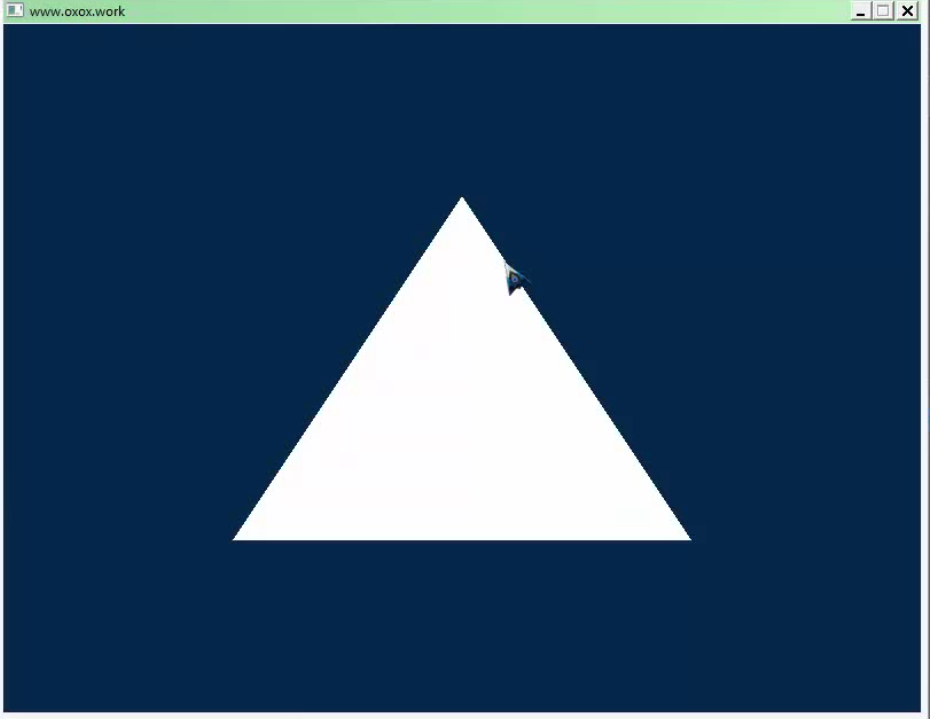
\includegraphics[scale = 0.5]{VBOMeshResult.png}
				\caption{上述Mesh代码绘画效果}
				\label{VAOResult}
			\end{figure}
	
	\subsection{光照添加}
	
	\subsection{纹理添加}
		

\chapter{MFC with OpenGL}
	\section{环境配置}
		\url{http://blog.csdn.net/sircarfield/article/details/6992586}
		
		\url{http://www.cnblogs.com/phinecos/archive/2007/07/28/834916.html}
		
	\section{闪烁解决办法}
		\url{http://blog.sina.com.cn/s/blog_6d4b374e010141ix.html}
		    
		\url{http://bbs.csdn.net/topics/390804673}
			
	\section{定时器概念与程序}
		\url{http://blog.sina.com.cn/s/blog_678e97f80100thp7.html}
			
			
	\section{坐标确定}
		左下角为原点
		
	\section{画椭球}
		\url{http://www.tuicool.com/articles/zmE3Mr}
		

\chapter{OpenGL 读取 OBJ 文件}
    \section{参考文献} 
		\subparagraph{OBJ 文件格式}\url{http://guanser.blog.163.com/blog/static/2112467872012877161702/}
	
	
 
\chapter{OpenGL 实现天空盒子}
	\section{实现}
		
	\section{错误记录}
		\paragraph{1.error LNK1281}error LNK1281: 无法生成 SAFESEH 映像VS2013常见编译错误解决
		
		\subparagraph{解决方案}:
		
		打开项目属性的链接器的命令行,在那里输入: /SAFESEH:NO点击确定再次编译,成功解决问题


\chapter{PCL  安装}
	\section{错误记录}
		\paragraph{1.error LNK2019} 要么是 依赖库没配置好, 要么就是32位与64位不兼容(这里包括 库与系统不兼容,还包括库与系统兼容但与编译器不兼容)
		
		如当使用 64位的库时,也是64位的系统,虽然你使用的编译器也是64位,但是在编译的时候并没有选择 x64,而选择了win32 也会出现这个错误
		
		参考该文章的更改编译器部分\url{http://www.ithao123.cn/content-8701571.html}
\end{document} 
 		    